\documentclass[journal,12pt,onecolumn]{IEEEtran}

%--- PREAMBLE ---
% Workaround for conflict between amsmath and txfonts
\let\negmedspace\undefined
\let\negthickspace\undefined

% --- PACKAGES ---
\usepackage[utf8]{inputenc} % Modern input encoding
\usepackage[T1]{fontenc}    % Font encoding for better output
\usepackage{cite}
\usepackage{amsmath,amssymb,amsfonts,amsthm}
\usepackage{algorithmic}
\usepackage{graphicx}
\graphicspath{{./figs/}}
\usepackage{textcomp}
\usepackage{xcolor}
\usepackage{txfonts}
\usepackage{listings}
\usepackage{enumitem}
\usepackage{mathtools}
\usepackage{gensymb}
\usepackage{comment}
\usepackage{caption}
\usepackage{tkz-euclide}
\usepackage{gvv} % Note: This is a non-standard package and requires gvv.sty file
\usepackage{xparse}
\usepackage{array}
\usepackage{longtable}
\usepackage{calc}
\usepackage{multirow}
\usepackage{multicol}
\usepackage{hhline}
\usepackage{ifthen}
\usepackage{lscape}
\usepackage{tabularx}
\usepackage{float}
\usepackage{textcomp}
\usepackage{subfigure}

\usepackage[breaklinks=true]{hyperref} % Should be loaded last
 \usepackage{newunicodechar}
\newunicodechar{₹}{\rupee}

% --- THEOREM DEFINITIONS & CUSTOM COMMANDS ---
\newtheorem{theorem}{Theorem}[section]
\newtheorem{problem}{Problem}
\newtheorem{proposition}{Proposition}[section]
\newtheorem{lemma}{Lemma}[section]
\newtheorem{corollary}[theorem]{Corollary}
\newtheorem{example}{Example}[section]
\newtheorem{definition}[problem]{Definition}
\theoremstyle{remark}

\begin{document}

% --- TITLE & AUTHOR ---
\title{GATE 2012 BT}
\author{EE25BTECH11014 - BHOOMIKA LOKESH}
\maketitle

% Note: The following commands change the numbering of all figures and tables
% to match the main question counter. This can be fragile.
\renewcommand{\thefigure}{\theenumi}
\renewcommand{\thetable}{\theenumi}

\section{Q.1-Q.5 carry one mark each}
\begin{enumerate}
\item In mismatch correction repair, the parental DNA strand is distinguished from the daughter strand by
\begin{multicols}{4}
\begin{enumerate}
\item acetylation
\item phosphorylation
\item methylation
\item glycosylation
\end{enumerate}
\end{multicols} \hfill(GATE 2012 BT)

\item  The basis for blue-white screening with pUC vectors is
\begin{multicols}{4}
\begin{enumerate}
\item intraallelic complementation
\item  intergenic complementation
\item  intragenic suppression	
\item  extragenic suppression
\end{enumerate}
\end{multicols} \hfill(GATE 2012 BT)

    \item Idiotypic determinants of an antibody are associated with the
\begin{multicols}{2}
\begin{enumerate}
\item 	constant region of the heavy chains
\item  constant region of the light chains
\item  variable region	
\item  constant regions of light and heavy chains
\end{enumerate}
\end{multicols} \hfill(GATE 2012 BT)

\item 	Identification of blood groups involves
\begin{multicols}{4}
\begin{enumerate}
\item	precipitation	
\item  neutralization
\item opsonization
\item  agglutination
\end{enumerate}
\end{multicols} \hfill(GATE 2012 BT)

\item 	B-lymphocytes originate from the bone marrow whereas T-lymphocytes originate from
\begin{multicols}{4}
\begin{enumerate}
\item thymus	
\item  bone marrow	
\item  spleen	
\item  liver
\end{enumerate}
\end{multicols} \hfill(GATE 2012 BT)

\item 	A humanized antibody is one in which the
\begin{multicols}{2}
\begin{enumerate}
\item	heavy and light chains are from human
\item heavy chain is from human and light chain is from mouse
\item 	light chain is from human and heavy chain is from mouse
\item 	CDRs are from mouse, and the rest is from human
\end{enumerate}
\end{multicols} \hfill(GATE 2012 BT)

\item 	Dimethyl sulfoxide (DMSO) is used as a cryopreservant for mammalian cell cultures because
\begin{multicols}{2}
\begin{enumerate}
\item	it is an organic solvent
\item 	it easily penetrates cells
\item 	it protects cells by preventing crystallization of water
\item 	it is also utilized as a nutrient
\end{enumerate}
\end{multicols} \hfill(GATE 2012 BT)

\item 	Nude mice refers to
\begin{multicols}{4}
\begin{enumerate}
\item mice without skin	
\item mice without thymus
\item knockout mice
\item transgenic mice
\end{enumerate}
\end{multicols} \hfill(GATE 2012 BT)

\item 	Heat inactivation of serum is done to inactivate
\begin{multicols}{4}
\begin{enumerate}
\item prions	
\item mycoplasma 
\item complement	
\item pathogenic bacteria
\end{enumerate}
\end{multicols} \hfill(GATE 2012 BT)


\item Choose the correct signal transduction pathway.

\begin{enumerate}
\item$ Hormone \rightarrow 7 TM receptor\rightarrow G protein \rightarrow cAMP \rightarrow PKA$
\item $Hormone \rightarrow G protein \rightarrow 7 TM receptor \rightarrow cAMP \rightarrow PKA$
\item $Hormone \rightarrow 7 TM receptor \rightarrow G protein \rightarrow PKA \rightarrow cAMP$
\item $Hormone \rightarrow 7 TM receptor \rightarrow cAMP \rightarrow G protein \rightarrow PKA$
\end{enumerate} \hfill(GATE 2012 BT)



\item 	A protein is phosphorylated at a serine residue. A phosphomimic mutant of the protein can be generated by substituting that serine with
\begin{multicols}{4}
\begin{enumerate}
\item  glycine	
\item  alanine	
\item  aspartate	
\item  threonine
\end{enumerate}
\end{multicols} \hfill(GATE 2012 BT)

\item A truncated polypeptide is synthesized due to a nonsense mutation. Where would you introduce another mutation to obtain a full-length polypeptide?
\begin{multicols}{2}
\begin{enumerate}
\item 	Ribosomal protein gene
\item  Transfer RNA gene
\item  DNA repair gene	
\item  Ribosomal RNA gene
\end{enumerate}
\end{multicols} \hfill(GATE 2012 BT)

\item Protein-DNA interactions in vivo can be studied by
\begin{multicols}{2}
\begin{enumerate}
\item 	gel shift assay 
\item  Southern hybridization
\item  chromatin immunoprecipitation assay	
\item  fluorescence in situ hybridization assay
\end{enumerate}
\end{multicols} \hfill(GATE 2012 BT)

\item The direction of shell coiling in the snail Limnaea peregra is a classic example of
\begin{multicols}{2}
\begin{enumerate}
\item	chromosomal inheritance	
\item  extra-chromosomal inheritance
\item  chromosomal translocation	
\item  homologous recombination
\end{enumerate}
\end{multicols} \hfill(GATE 2012 BT)


\item During photorespiration under low $CO_{2}$ and high $O_2$ levels, $O_2$ reacts with ribulose 1,5- bisphosphate to yield
\begin{enumerate}
\item	one molecule each of 3-phosphoglycerate and 2-phosphoglycolate
\item 	two molecules of 3-phosphoglycerate
\item 	two molecules of 2-phosphoglycolate
\item 	one molecule each of 3-phosphoglycerate and glyoxylate
\end{enumerate} \hfill(GATE 2012 BT)

\item 	Which one of the following is \textbf{NOT} a protoplast fusion inducing agent?
\begin{multicols}{2}
\begin{enumerate}
\item	Inactivated Sendai virus	
\item  $Ca^{2+}$ at alkaline pH
\item  Polyethylene glycol
\item  Colchicine
\end{enumerate}
\end{multicols} \hfill(GATE 2012 BT)


\item The activity of an enzyme is expressed in International Units (IU). However, the S.I. unit for enzyme activity is Katal. One Katal is
\begin{multicols}{4}
\begin{enumerate}
\item $1.66 × 10^{4}$ IU	
\item  $60$ IU	
\item  $6 × 10^7$ IU	
\item  $10^{6}$ IU
\end{enumerate}
\end{multicols} \hfill(GATE 2012 BT)


\item 	Identify the statement that is NOT applicable to an enzyme catalyzed reaction.
\begin{enumerate}
\item	Enzyme catalysis involves propinquity effects
\item 	The binding of substrate to the active site causes a strain in the substrate
\item 	Enzymes do not accelerate the rate of reverse reaction
\item 	Enzyme catalysis involves acid-base chemistry
\end{enumerate}  \hfill(GATE 2012 BT)

\item An example of a derived protein structure database is
\begin{multicols}{4}
\begin{enumerate}
\item Pfam
\item SCOP	
\item GEO	
\item Prosite
\end{enumerate}
\end{multicols} \hfill(GATE 2012 BT)


\item 	An example of a program for constructing a phylogenetic tree is
\begin{multicols}{4}
\begin{enumerate}
\item phylip	
\item  phrap	
\item  prodom	
\item  PHDsec
\end{enumerate}
\end{multicols} \hfill(GATE 2012 BT)

\item 	Synteny refers to
\begin{multicols}{2}
\begin{enumerate}
\item 	gene duplication from a common ancestor
\item 	a tree representation of related sequences
\item 	the extent of similarity between two sequences
\item 	local conservation of gene order
\end{enumerate}
\end{multicols} \hfill(GATE 2012 BT)

\item 	While searching a database for similar sequences, E value does NOT depend on the
\begin{enumerate}
\item 	sequence length	
\item  number of sequences in the database
\item  scoring system
\item  probability from a normal distribution
\end{enumerate} \hfill(GATE 2012 BT)

\item 	In transmission electron microscopy, electron opacity is greatly enhanced by treating the specimen with
\begin{multicols}{2}
\begin{enumerate}
\item	ferrous ammonium sulfate	
\item  uranium acetate
\item  sodium chloride	
\item  basic fuchsin
\end{enumerate}
\end{multicols} \hfill(GATE 2012 BT)

\item The molarity of water in a water : ethanol mixture (15 : 85, v/v) is approximately
\begin{multicols}{4}
\begin{enumerate}
\item $0.85$	
\item  $5.55$
\item  $8.5$
\item  $55.5$
\end{enumerate}
\end{multicols} \hfill(GATE 2012 BT)

\item The helix content of a protein can be determined using
\begin{multicols}{2}
\begin{enumerate}
\item	an infrared spectrometer	
\item a fluorescence spectrometer
\item a circular dichroism spectrometer	
\item a UV-Visible spectrophotometer
\end{enumerate}
\end{multicols} \hfill(GATE 2012 BT)

\section{Q. 26 to Q. 55 carry two marks each.}
\item Which one of the following DNA sequences carries an invert repeat?
\begin{enumerate}
\item	ATGAGCCCCGAGTA TACTCGGGGCTCAT
\item  ATGAGCCGAGCCTA ACTCGGCTCGGAT
\item ATGAGCCGGCTCTA TACTCGGCCGAGAT
\item  ATGAGCCTATGGTA TACTCGGATACCAT
\end{enumerate}
 
\item 	In zinc finger proteins, the amino acid residues that coordinate zinc are
\begin{multicols}{4}
\begin{enumerate}
\item	Cys and His	
\item  Asp and Glu
\item  Arg and Lys	
\item  Asp and Arg
\end{enumerate}
\end{multicols} \hfill(GATE 2012 BT)

\item 	Match the entries in Group I with those in Group II.\\
\begin{tabular}{c c}
\textbf{Group I}&	\textbf{Group II}\\
P.	MTT	1.& 	Dihydrofolate reductase\\
Q.	Annexin V&	2.	Succinate dehydrogenase\\
R.	Methotrexate&	3.	Microtubules\\
S.	Taxol&	4.	Phosphatidylserine
\end{tabular}
\begin{multicols}{4}
\begin{enumerate}
\item	P-3, Q-1, R-4, S-2
\item  P-2, Q-4, R-1, S-3
\item  P-2, Q-3, R-4, S-1
\item  P-4, Q-2, R-1, S-3
\end{enumerate}
\end{multicols} \hfill(GATE 2012 BT)


\item In an exponentially growing batch culture of Saccharomyces cerevisiae, the cell density is 20 $gl^{-1}$ \brak{DCW}, the specific growth rate ($\mu$) is $0.4 h{-1}$ and substrate uptake rate ($\mu$)  is 16 $gl^{-1}h^{-1}$. The cell yield coefficient $Y_{x/s}$ will be
\begin{multicols}{4}
\begin{enumerate}
\item $0.32$	
\item  $0.64$	
\item  $0.80$	
\item  $0.50$
\end{enumerate}
\end{multicols} \hfill(GATE 2012 BT)



\item 	A single base pair of DNA weighs $1.1 × 10^{-21}$ grams. How many picomoles of a plasmid vector of length 2750 bp are contained in 1 $\mu$g of purified DNA?
\begin{multicols}{4}
\begin{enumerate}
\item  $0.30$	
\item $0.55$
\item  $0.25$	
\item  $0.91$
\end{enumerate}
\end{multicols} \hfill(GATE 2012 BT)

\item 	Match the terms in Group I with the ploidy in Group II.

    \begin{tabular}{c c}
    Group I&	Group II\\
P.	Disome	&1.	2n + 1\\
Q.	Monosome&	2.	2n – 1\\
R.	Nullisome&	3.	n – 1\\
S.	Trisome	&4.	n + 1
  \end{tabular}

\begin{multicols}{2}
\begin{enumerate}
\item P-4, Q-2, R-3, S-1	
\item  P-4, Q-3, R-1, S-2
\item  P-2, Q-3, R-4, S-1
\item  P-1, Q-4, R-3, S-2
\end{enumerate}
\end{multicols} \hfill(GATE 2012 BT)

\item What is the rank of the following matrix?\\
 A=\myvec{5 & 3 & -1\\
         6 & 2 & -4\\
         14 & 10 & 0 } 

\item Match the products in Group I with the applications in Group II.\\
    \begin{tabular}{c c}
    Group I&	Group II\\
P.	Digoxin	&1.	Muscle relaxant\\
Q.	Stevioside	&2.	Anti-cancer agent\\
R.	Atropine	&3.	Cardiovascular disorder\\
S.	Vinblastine	&4.	Sweetener
\end{tabular}
\begin{multicols}{2}
\begin{enumerate}
\item 	P-1, Q-4, R-3, S-2
\item P-3, Q-2, R-1, S-4
\item  P-3, Q-4, R-1, S-2	
\item  P-2, Q-3, R-1, S-4
\end{enumerate}
\end{multicols} \hfill(GATE 2012 BT)



\item Determine the correctness or otherwise of the following Assertion \brak{a} and Reason \brak{r}.\\

Assertion: The production of secondary metabolites in plant cell cultures is enhanced by the addition of elicitors.\\
Reason:	Elicitors induce the expression of enzymes responsible for the biosynthesis of secondary metabolites.
\begin{enumerate}
\item 	Both \brak{a} and \brak{r} are true but \brak{r} is not the correct reason for \brak{a}
\item 	Both \brak{a} and \brak{r} are true and \brak{r} is the correct reason for \brak{a}
\item 	\brak{a} is true but \brak{r} is false
\item 	\brak{a} is false but \brak{r} is true
\end{enumerate}

\item Determine the correctness or otherwise of the following Assertion \brak{a} and Reason \brak{r}.\\

Assertion: Plants convert fatty acids into glucose.\\
Reason:	Plants have peroxisomes.
\begin{enumerate}
\item 	Both \brak{a} and \brak{r} are true but \brak{r} is not the correct reason for \brak{a}
\item 	Both \brak{a} and \brak{r} are true and \brak{r} is the correct reason for \brak{a}
\item \brak{a} is true but \brak{r} is false
\item 	\brak{a} is false but \brak{r} is true
\end{enumerate}


\item Determine the correctness or otherwise of the following Assertion \brak{a} and Reason \brak{r}.\\

Assertion: In direct somatic embryogenesis, embryos are developed without going through callus formation.\\
Reason:	This is possible due to the presence of pre-embryonically determined cells.
\begin{enumerate}
\item Both \brak{a} and \brak{r} are true but \brak{r} is not the correct reason for \brak{a}
\item \brak{a} is false but \brak{r} is true
\item \brak{a} is true but \brak{r} is false
\item Both \brak{a} and \brak{r} are true and \brak{r} is the correct reason for \brak{a}
\end{enumerate}

\item Match the entries in Group I with the process parameters in Group II.\\
  \begin{tabular}{c c}
    Group I&	Group II\\
P.	Clark electrode &	1.	Liquid level\\
Q.	Redox probe	& 2.	Dissolved oxygen concentration\\
R.	Load cell	& 3.	Vessel pressure\\
S.	Diaphragm gauge	&4.	pH (anaerobic process)\\
\end{tabular}
\begin{multicols}{2}
\begin{enumerate}
\item P-2, Q-1, R-3, S-4	
\item  P-4, Q-2, R-3, S-1
\item  P-2, Q-4, R-1, S-3
\item  P-2, Q-1, R-4, S-3
\end{enumerate}
\end{multicols} \hfill(GATE 2012 BT)


\item 	Match the downstream processes in Group I with the products in Group II.\\

 \begin{tabular}{c c}
    Group I&	Group II\\
P.	Solvent extraction	&1.	Lactic acid\\
Q.	Protein-A linked affinity chromatography&	2.	Penicillin\\
R.	Extractive distillation	&3.	Monoclonal antibody\\
S.	Salting out	&4.	Lipase
\end{tabular}
\begin{multicols}{2}
\begin{enumerate}
\item P-2, Q-3, R-1, S-4	
\item P-4, Q-1, R-2, S-3
\item P-4, Q-1, R-3, S-2
\item P-2, Q-4, R-1, S-3
\end{enumerate}
\end{multicols} \hfill(GATE 2012 BT)

\item Determine the correctness or otherwise of the following Assertion \brak{a} and Reason \brak{r}.\\

Assertion: Cell mass yield of a methylotrophic yeast is more on methanol compared to glucose.\\
Reason:	Methanol has a greater degree of reductance compared to glucose.
\begin{multicols}{2}
\begin{enumerate}
\item	Both \brak{a} and \brak{r} are correct and \brak{r} is the correct reason for \brak{a}
\item 	\brak{a} is correct, \brak{r} is false
\item 	\brak{a} is false, \brak{r} is correct
\item 	Both \brak{a} and \brak{r} are correct but \brak{r} is not the correct reason for \brak{a}
\end{enumerate}
\end{multicols} \hfill(GATE 2012 BT)

\item 	A disease is inherited by a child with a probability of $1/4$. In a family with two children, the probability that exactly one sibling is affected by this disease is
\begin{multicols}{4}
\begin{enumerate}
\item $\frac{1}{4}$ 	
\item $\frac{3}{8}$
\item $\frac{7}{16}$
\item $\frac{9}{16}$
\end{enumerate}
\end{multicols} \hfill(GATE 2012 BT)

 
\item Match the organisms in Group I with the entries in Group II.\\

 \begin{tabular}{c c}
    Group I&	Group II\\
P.	Clostridium	&1.	Rods with teichoic acid in the cell wall\\
Q.	Escherichia	&2.	Rods with endospores\\
R.	Vibrio	&3.	Helical rods with flagella\\
S.	Bacillus	&4.	Rods with LPS in the outer membrane\\
&5.	Curved rods with polar flagella
\end{tabular}
\begin{multicols}{4}
\begin{enumerate}
\item	P-2, Q-4, R-5, S-1
\item  P-2, Q-1, R-5, S-4
\item  P-5, Q-4, R-2, S-3	
\item  P-3, Q-2, R-1, S-4
\end{enumerate}
\end{multicols} \hfill(GATE 2012 BT)

\item Match the entries in Group I with the methods of sterilization in Group II.\\
\begin{tabular}{c c}
    Group I&	Group II\\
P.	Serum	&1.	Autoclave\\
Q.	Luria broth	&2.	Membrane filtration\\
R.	Polypropylene tubes&	3.	UV irradiation\\
S.	Biological safety cabinets&	4.	Gamma irradiation\\
&5.	Dry heat
\end{tabular}
\begin{multicols}{4}
\begin{enumerate}
\item P-5, Q-3, R-1, S-4	
\item  P-1, Q-4, R-5, S-3
\item  P-2, Q-1, R-4, S-3	
\item  P-4, Q-1, R-3, S-5
\end{enumerate}
\end{multicols} \hfill(GATE 2012 BT)


\item Match the high energy compounds in Group I with the biosynthetic pathways for the molecules in
Group II.\\
\begin{tabular}{c c}

Group I&	Group II\\
P.	GTP	&1.	Fatty acid\\
Q.	UTP	&2.	Phospholipid\\
R.	CTP	&3.	Protein\\
S.	Acyl coenzyme A	&4.	Peptidoglycan\end{tabular}
\begin{multicols}{4}
\begin{enumerate}
\item P-3, Q-2, R-4, S-1	
\item  P-2, Q-4, R-3, S-1
\item P-4, Q-3, R-1, S-2	
\item  P-3, Q-4, R-2, S-1
\end{enumerate}
\end{multicols} \hfill(GATE 2012 BT)


\item Match the vitamins in Group I with the processes/reactions in Group II.\\
\begin{tabular}{c c}

Group I	&Group II\\
P.	Pantothenic acid	&1.	Electron transport\\
Q.	Vitamin B2	&2.	Transfer of 1-C units\\
R.	Vitamin B6	&3.	Decarboxylation\\
S.	Folic acid	&4.	Fatty acid metabolism\\
&5.	Hydrolysis\end{tabular}
\begin{multicols}{4}
\begin{enumerate}
\item	P-5, Q-2, R-4, S-1	
\item  P-4, Q-1, R-3, S-2
\item  P-4, Q-2, R-1, S-3	
\item P-2, Q-1, R-3, S-5
\end{enumerate}
\end{multicols} \hfill(GATE 2012 BT)

\item Consider the data set $14, 18, 14, 14, 10, 29, 33, 31, 25$. If you add $20$ to each of the values, then
\begin{multicols}{2}
\begin{enumerate}
\item	both mean and variance change	
\item  both mean and variance are unchanged
\item  the mean is unchanged, variance changes	
\item  the mean changes, the variance is unchanged
\end{enumerate}
\end{multicols} \hfill(GATE 2012 BT)


\item An enzymatic reaction is described by the following rate expression.\\
$ v=\dfrac{V_mS}{k_m+S+S^2/k_s}$
Which one of the following curves represents this expression?\\
\begin{multicols}{2}
\begin{enumerate}[label=\alph*)]

\item 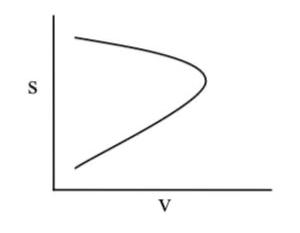
\includegraphics[width=0.4\columnwidth]{figures_3/fig_3.1.jpeg}
\item 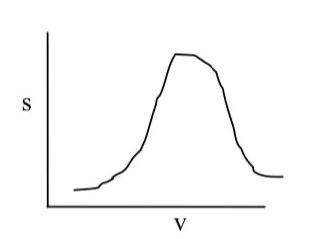
\includegraphics[width=0.4\columnwidth]{figures_3/fig_3.2.jpeg}
\item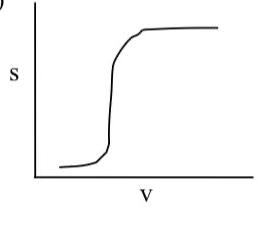
\includegraphics[width=0.4\columnwidth]{figures_3/fig_3.3.jpeg} 
\item 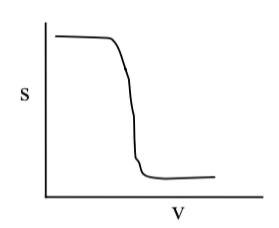
\includegraphics[width=0.4\columnwidth]{figures_3/fig_3.4.jpeg}
\end{enumerate}
\end{multicols} \hfill(GATE 2012 BT)


\item A bacterial culture ($200 \mu l$ containing $1.8 × 10^9$ cells) was treated with an antibiotic Z ($50 \mu $g per ml) for 4 h at $37^\circ C$. After this treatment, the culture was divided into two equal aliquots.
Set A: 100 $\mu$l was plated on Luria agar.
Set B: 100 $\mu$l was centrifuged, the cell pellet washed and plated on Luria agar.
After incubating these two plates for $24 $h at  $37^\circ C$, Set A plate showed no colonies, whereas the Set B plate showed 0.9 × 109 cells. This experiment showed that the antibiotic Z is
\begin{multicols}{2}
\begin{enumerate}
\item	bacteriostatic
\item  bacteriocidal
\item  bacteriolytic	
\item apoptotic
\end{enumerate}
\end{multicols} \hfill(GATE 2012 BT)


\section{Common Data Questions}
\textbf{Common Data for Questions 48 and 49 :}

In a muscle, the extracellular and intracellular concentrations of $Na^+$ are 150 mM and $12$ mM, and those of $K^+$ are $2.7$ mM and $140$ mM, respectively. Assume that the temperature is $25^\circ C$ and that the membrane potential is $-60$ mV, with the interior more negatively charged than the exterior. ($R = 8.314 J mol^{-1} K^{-1}$; $F = 96.45 kJ mol^{-1} V^{-1}$)
\item 	The free energy change for the transport of three Na+ out of the cell is
\begin{multicols}{4}
\begin{enumerate}
\item $+1.5$ kJ/mol	
\item $+17.4 $kJ/mol	
\item  $+18.9$ kJ/mol	
\item  $+36.3$ kJ/mol
\end{enumerate}
\end{multicols} \hfill(GATE 2012 BT)

\item The free energy change for the transport of two K+ into the cell is
\begin{multicols}{4}
\begin{enumerate}
\item $+8.0$ kJ/mol	
\item $+11.6$ kJ/mol	
\item $ +19.6$ kJ/mol	
\item  $+31.2$ kJ/mol
\end{enumerate}
\end{multicols} \hfill(GATE 2012 BT)

\textbf{Common Data for Questions 50 and 51:}\\
The purification data for an enzyme is given below:\\
\begin{tabular}{|c|c|c|c|c|c|}
\hline
 &Step&	Volume(ml)	&Total protein (mg)&	Total activity(Units )& Specific activity(Units/mg)\\
 \hline
P	&Cell-free extract&	17&	177&	102 &0.58\\
\hline
Q	&Q- Sepharose	&14&	18.8&	72&	3.83\\
\hline
R	&Phenyl Sepharose	&26&	9.2&	45&	4.89\\
\hline
S	&Sephacryl S-200&	7	&4.1	&30	&7.32\\
\hline
\end{tabular}

\item The fold purification for each step is
\begin{multicols}{2}
\begin{enumerate}
\item P-0.1, Q- 0.66, R-0.84,S- 1.26
\item P-1.0, Q-0.52, R-0.67, S-0.8
\item P-1, Q-6.6, R-8.4, S-12.6	
\item P-100, Q-66, R-84, S-12
\end{enumerate}
\end{multicols} \hfill(GATE 2012 BT)

\item 	The yield \brak{\%} for each step is
\begin{multicols}{2}
\begin{enumerate}
\item  P-10, Q-7.2, R-4.5, S-2.0	
\item  P-34, Q-24, R-15, S-1
\item  P-3.4, Q-2.4, R-1.5, S-0.1
\item  P-100, Q-71, R-44, S-29
\end{enumerate}
\end{multicols} \hfill(GATE 2012 BT)


\textbf{Linked Answer Questions}

\textbf{Statement for Linked Answer Questions 52 and 53:}
An \textit{E. coli} cell of volume $10^{-12} cm^{3}$ contains $60$ molecules of lac-repressor. The repressor has a binding affinity (Kd) of 10-8 M and $10^{-9}$ M with and without lactose respectively, in the medium.\\
\item 	The molar concentration of the repressor in the cell is
\begin{multicols}{2}
\begin{enumerate}
\item $ 0.1$ nM	
\item  $1$ nM	
\item  $10$ nM	
\item  $100$ nM
\end{enumerate}
\end{multicols} \hfill(GATE 2012 BT)


\item Therefore the lac-operon is
\begin{multicols}{2}
\begin{enumerate}
\item repressed and can only be induced with lactose.
\item 	repressed and cannot be induced with lactose.
\item 	not repressed.
\item 	expressed only when glucose and lactose are present.
\end{enumerate}
\end{multicols} \hfill(GATE 2012 BT)


\textbf{Statement for Linked Answer Questions 54 and 55:}

$\beta$ Galactosidase bound to DEAE-cellulose is used to hydrolyze lactose to glucose and galactose in a plug flow bioreactor with a packed bed of volume 100 liters and a voidage $\brak{\epsilon}$ of $0.55$. The $K'_m$ and $V'_max$ for the immobilized enzyme are $0.72$ $gl^{-1}$ and $18 gl^{-1}h^{-1}$, respectively. The lactose concentration in the field stream is $20 gl^{-1}$, and a fractional conversion of $0.90$ is desired. Diffusional limitations may be ignored.\\
\item The residence time required for the steady state reactor operation will be
\begin{multicols}{4}
\begin{enumerate}
\item $0.1$ h	
\item $0.4$ h	
\item $1.0$ h	
\item  $1.1$ h
\end{enumerate}
\end{multicols} \hfill(GATE 2012 BT)

\item The feed flow rate required for the above bioconversion will be
\begin{multicols}{4}
\begin{enumerate}
\item  $50 lh^{-1}$	
\item  $55lh^{-1}$
\item  $137lh^{-1}$	
\item  $550lh^{-1}$
\end{enumerate}
\end{multicols} \hfill(GATE 2012 BT)



\section{General Aptitude (GA) Questions}
\textbf{Q.56– Q. 60 carry one mark each}.
\item 	The cost function for a product in a firm is given by $5q^{2}$, where q is the amount of production. The firm can sell the product at a market price of Rs.50 per unit. The number of units to be produced by the firm such that the profit is maximized is
\begin{multicols}{4}
\begin{enumerate}
\item  5	
\item  10	
\item  15
\item  25
\end{enumerate}
\end{multicols} \hfill(GATE 2012 BT)


\item Choose the most appropriate alternative from the options given below to complete the following sentence:

Suresh’s dog is the one\rule{2cm}{0.4pt} \textbf{was hurt in the stampede.}
\begin{multicols}{4}
\begin{enumerate}
\item  that	
\item  which
\item  who
\item  whom
\end{enumerate}
\end{multicols} \hfill(GATE 2012 BT)


\item Choose the grammatically\textbf{ INCORRECT} sentence:

\begin{enumerate}
\item	They gave us the money back less the service charges of Three Hundred rupees.
\item 	This country’s expenditure is not less than that of Bangladesh.
\item 	The committee initially asked for a funding of Fifty Lakh rupees, but later settled for a lesser sum.
\item 	This country’s expenditure on educational reforms is very less.
\end{enumerate}

\item 	Which one of the following options is the closest in meaning to the word given below?\
\textbf{Mitigate}
\begin{multicols}{4}
\begin{enumerate}
\item Diminish	
\item  Divulge	
\item  Dedicate	
\item  Denote

\end{enumerate}
\end{multicols} \hfill(GATE 2012 BT)

\item Choose the most appropriate alternative from the options given below to complete the following sentence:\\

\textbf{Despite several\rule{2cm}{0.4pt}the mission succeeded in its attempt to resolve the conflict.}
\begin{multicols}{4}
\begin{enumerate}
\item attempts	
\item  setbacks
\item  meetings
\item  delegations
\end{enumerate}
\end{multicols} \hfill(GATE 2012 BT)


\textbf{Q.61- Q. 65 carry two marks each.}
\item \textbf{Wanted Temporary, Part-time persons for the post of Field Interviewer to conduct personal interviews to collect and collate economic data. Requirements: High School-pass, must be available for Day, Evening and Saturday work. Transportation paid, expenses reimbursed.}\\
Which one of the following is the best inference from the above advertisement?
\begin{multicols}{2}
\begin{enumerate}
\item	Gender-discriminatory
\item 	Xenophobic
\item 	Not designed to make the post attractive
\item 	Not gender-discriminatory
\end{enumerate}
\end{multicols} \hfill(GATE 2012 BT)

\item Given the sequence of terms, AD CG FK JP, the next term is
\begin{multicols}{2}
\begin{enumerate}
\item OV	
\item OW	
\item  PV	
\item  PW
\end{enumerate}
\end{multicols} \hfill(GATE 2012 BT)

 
\item Which of the following assertions are \textbf{CORRECT}?\\
P: Adding 7 to each entry in a list adds 7 to the mean of the list\\
Q: Adding 7 to each entry in a list adds 7 to the standard deviation of the list R: Doubling each entry in a list doubles the mean of the list\\
S: Doubling each entry in a list leaves the standard deviation of the list unchanged
\begin{multicols}{4}
\begin{enumerate}
\item P, Q	
\item  Q, R	
\item  P, R	
\item  R, S
\end{enumerate}
\end{multicols} \hfill(GATE 2012 BT)


\item 	An automobile plant contracted to buy shock absorbers from two suppliers X and Y. X supplies $60\%$ and Y supplies $40\%$ of the shock absorbers. All shock absorbers are subjected to a quality test. The ones that pass the quality test are considered reliable. Of X’s shock absorbers, $96\%$ are reliable. Of Y’s shock absorbers, $72\%$ are reliable.\\

The probability that a randomly chosen shock absorber, which is found to be reliable, is made by Y is
\begin{multicols}{4}
\begin{enumerate}
\item $0.288$	
\item $0.334$
\item $0.667$	
\item $0.720$
\end{enumerate}
\end{multicols} \hfill(GATE 2012 BT)


\item 	A political party orders an arch for the entrance to the ground in which the annual convention is being held. The profile of the arch follows the equation $y = 2x – 0.1x^2$ where y is the height of the arch in meters. The maximum possible height of the arch is
\begin{multicols}{4}
\begin{enumerate}
\item $8$ meters	
\item  $10$ meters	
\item  $12$ meters	
\item  $14$ meters
\end{enumerate}
\end{multicols} \hfill(GATE 2012 BT)

\centering
\textbf{END OF THE QUESTION PAPER}




\end{enumerate}
\end{document}
